\documentclass[a4paper, amsmath]{oblivoir}

\usepackage{fapapersize}
\usefapapersize{*,*,1in,*,1in,*}
\usepackage[default=false,exception={vmatrix}]{ob-mathleading}
\usepackage{mathtools}
\usepackage{listings}
\usepackage{xcolor}

\newcommand\pkg[1]{\textsf{#1}}

\usepackage{tcolorbox}
\tcbuselibrary{listings,breakable}
\usepackage{blindtext}

\begin{document}

\title{기호식품 가격 인상과 삶의 질에 대한 상관관계 분석}
\author{홍길동(hong@pusan.ac.kr)}
\date{\today, v0.1.4}

\maketitle

\begin{abstract}
기호식품의 가격 인상이 삶의 질에 어떤 영향을 주는지 알아보고자 하는 것이 목적이며, 
기호식품 가격 인상과 삶의 질에 관한 가설을 설정하고 검증하는 과정을 간략하게 소개하는 것이 주요 목적이다.
\end{abstract}

\tableofcontents*

\section{서론}

경제성장과 생활 수준의 향상으로 더 나은 삶 또는 양질의 삶을 살아가고자 하는 시대가 되었다.
시대의 흐름에 발맞추어 흡연과 주류에 대한 경각심이 높아지고 있다. 
이를 억제하기 위해서 가격정책을 통한 수요를 제한 하기 위한 방안을 모색하였다. 
담배는 가격 인상과 광고 제한 등의 방법을 사용하여 수요를 제한하였고, 주류는 주류세 및 원가 상승으로 출고 가격을 인상하는 방법 등을 적용하였다.
하지만 이런 정책으로 흡연율은 낮아졌으나 반대로 한국담배공사(KT\&G)의 영업이익이 증가하게 되었고, 해당 정책이 세금 확보를 위한 인상이 아니냐는 의심을 받았다.
또한 주류세의 증가로 가계당 외식비용이 증가로 인해서, 외식에 대한 거부감과 경기 둔화 등이 겹쳐서 자영업에 위기가 오는 것이 아닌가 하는 우려도 함께 논의되고 있다.
이런 주장 혹은 가설을 검증하기 위해서 '한국 복지 패널(Korea Welfare Panel Study)'에서 총 17회의 패널 대상자를 통해 수집한 데이터를 사용하였다.
총 조사대상자는 118,422명으로 흡연과 주류에 대한 문항을 중심으로 진행하였다. 
삶의 질에 대한 계량적인 접근을 시도한 후에 집단별 임금(소득)수준을 고려하여 삶의 질을 상관관계를 파악하고 결과를 제시하고자 한다.

\begin{figure}
    \begin{center}    
    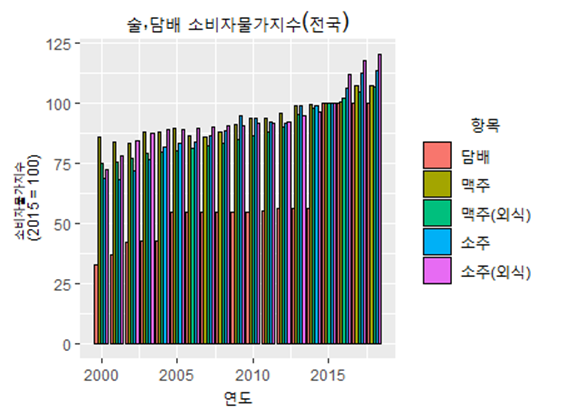
\includegraphics[width=0.8\linewidth]{./figz/image01.png}
    \end{center}    
    \caption{기호식품 가격인상과 소비자물가지수(전국)의 비교 }    
    \label{fig:long}    
    \label{fig:onecol}    
\end{figure}

\section{본론}
삶의 질에 관련된 문항은 리커트 척도(Likert scale)로 구성되어 있다. 
따라서 범주화된 집단을 분류하기 위해서 간단한 군집분석인 K-means을 활용하였다. 
군집 분석을 통해 삶의 질 수준을(만족도 최상위 그룹 ~ 만족도 최하위 그룹 : 5단계) 총 5가지로 구분하였다.

해당 분석에서는 군집으로 나뉘게 된 요인 중 중요도를 확인하고, 하나의 모델 식을 작성하기 위하여 실시하였으며 분석에 사용된 이론은 범주형 회귀분석(CATREG)을 사용하였다\cite{catreg2021}.
범주형 회귀분석(CATREG)은 범주에 숫자 값을 할당하고, 범주형 자료인 종속변수와 이를 설명해주는 독립변수 사이의 선형적인 관계를 보여주는 최적 선형 회귀 방정식을 작성하는 분석 방법이다.
해당 분석은 혼합형(범주형 및 순서형) 데이터를 동시에 척도화 함으로써 기존의 회귀분석을 확장하였다.
분석결과 삶의 질이 변화하는 데 가장 큰 기여도를 보인 요인은 건강만족도이며, 그 다음으로는 가족의 수입 만족도, 직업만족도, 여가생활 만족도, 주거환경 만족도, 가족관계만족도, 사회적 친분관계 만족도 순으로 중요한 기여도를 보이는 것을 확인 할 수 있다. 

\begin{figure}[!h]
    \begin{center}    
    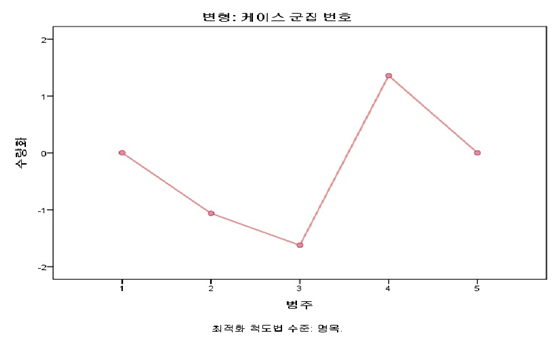
\includegraphics[width=0.8\linewidth]{./figz/image02.png}
    \end{center}    
    \caption{군집에 대한 범주형 회귀분석 내 수량화 도표}    
    \label{fig:long}    
    \label{fig:onecol}
\end{figure}

모든 독립변수의 회귀계수가 양의 값을 갖는 것을 고려하여 독립변수인 만족도 항목들의 수량화 도표를 보면, 기존 범주의 값이 커질수록 수량화 값도 같이 커지는 경향이 있다.
이는 독립변수가 5점 척도인 순서형 척도의 성질을 가지고 있어서, 만족도인 값이 증가할수록 수량화의 값도 증가하는 것으로 이해할 수도 있다.
이를 명목형 종속변수인 군집들과 비교를 해본다면, 독립변수의 만족도들이 증가할수록(5점으로 근사한다면), 군집은 4군집(만족도 최상위 그룹)에 근사한다는 것을 알 수 있고, 독립변수의 만족도들이 감소할수록(1점으로 근사한다면), 군집은 3군집(만족도 최하위그룹)으로 근사한다는 것을 알 수 있다.

\begin{figure}[!h]
    \begin{center}    
    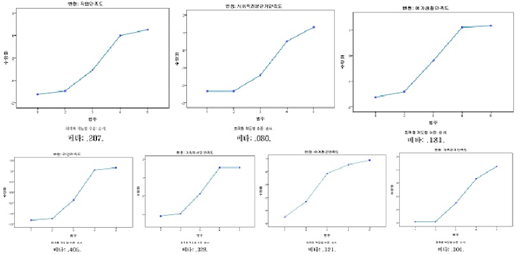
\includegraphics[width=0.8\linewidth]{./figz/image03.png}
    \end{center}    
    \caption{만족도 독립변수 대한 범주형 회귀분석 내 수량화 도표}    
    \label{fig:long}    
    \label{fig:onecol}    
\end{figure}

\section{결론}
분석과 시각화를 바탕으로 유해성 기호식품의 가격 상승이 삶의 질에 영향을 미치는지에 대한 결론은 '가격 상승과 삶의 질은 큰 관계가 없다'이다. 
연구 과정에서 삶의 질을 여러 구간으로 나누었고, 연도별로 비교해 보았을 때, 삶의 질의 변화에 큰 영향을 주는 요인이라면, 해당 기호식품의 가격의 변동이 있는 시기 근처와 해당 시기에 삶의 질의 변화는 많은 사람들이 비슷한 양상을 보여야 하고, 다양한 검증을 통해 변화의 양상에 대한 검증을 실시해야 하지만, 간단한 시각화 자료를 통해 살펴보아도 특정 시기에 많은 패널의 비슷한 변화 양상을 확인할 수 없었다.
이후 더욱 세분하여 변화있는 집단을 확인하고자 하였으나 이 역시 확인할 수 없었다. 따라서 본 연구를 통해 기호식품의 가격 인상은 삶의 질에 영향을 미치지 못한다고 할 수 있다. 

\bibliographystyle{unsrt}
\bibliography{references}

\end{document}